\documentclass[12pt]{article}

\title{An easy-to-implement numerical, visual method for generating the (non-)linear separating isosurface of two classes of objects in two-dimensional space using Marching Squares and OpenCV}
\author{
Shawn Halayka\footnote{Independent -- sjhalayka@gmail.com}
}


\date{\today\;\currenttime}

\usepackage{datetime}
\usepackage{listings}
\usepackage{cite}
\usepackage{xcolor}
\usepackage{graphicx}
\usepackage{setspace}
\usepackage{amsmath}
\usepackage{url}
\usepackage{amsfonts}
\usepackage{caption}
\usepackage{subcaption}

\usepackage[margin=1in]{geometry}

%\doublespace

\begin{document}




\maketitle

\begin{abstract}
With regard to the separating isosurface of two classes of objects in two-dimensional space, the transition from curvilinear to rectilinear is documented.
Marching Squares and OpenCV were used to calculate the data that were used for illustrations in this paper.
\end{abstract}




\section{Introduction}

In terms of statistical learning, a balance between high variance (curvilinearity) and high bias (rectilinearity) is to be had \cite{james}.

Marching Squares works as a radial (spherical) isosurface generator, as well as a rectilinear (planar) isosurface generator -- it all depends on the grid resolution.
The data generated by Marching Squares are the line segments that separate the two classes, as well as triangles for the area of each class.
Classifying a test point is a matter of ray-triangle intersection, which can be accelerated using a Bounding Volume Hierarchy or quadtree data structure.

OpenCV was used to downsize images.
OpenCV was also used to blur images.


\section{Conclusion}

Test...



\pagebreak


\begin{thebibliography}{9}

\bibitem{james} James, et al. An Introduction to Statistical Learning with Applications in R. ISBN: 978-1-0716-1417-4

\end{thebibliography}



\pagebreak





\begin{figure} 
\centering
  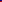
\includegraphics[width = 3 in]{2_res_image.png}
  \caption{Bitmap image used as input to the Marching Squares algorithm.
Image size is 2x2.
}
\end{figure}


\begin{figure} 
\centering
  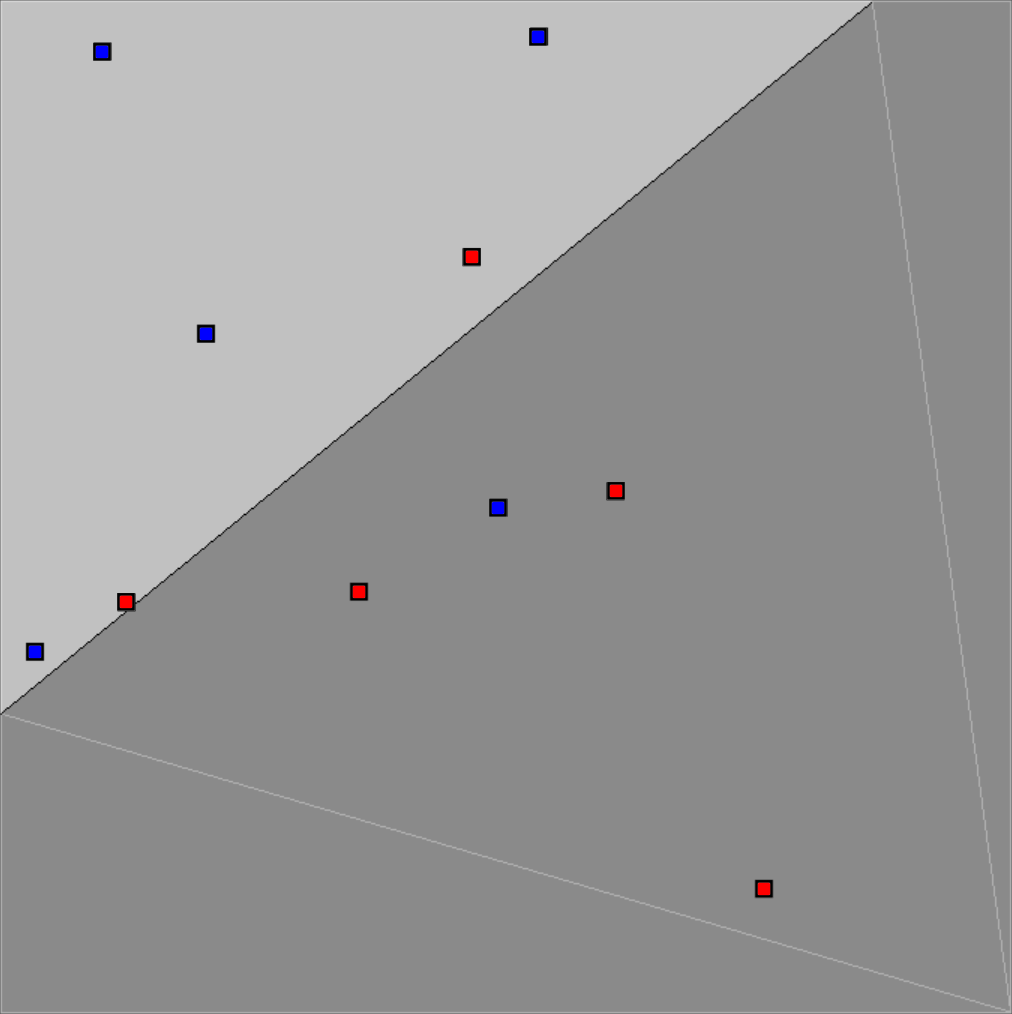
\includegraphics[width = 3 in]{2_res.png}
  \caption{The output of the Marching Squares algorithm: rectilinear separation. Grid resolution is 2x2.
}
\end{figure}






\begin{figure} 
\centering
  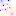
\includegraphics[width = 3 in]{16_res_image.png}
  \caption{Bitmap image used as input to the Marching Squares algorithm.
Image size is 16x16.
Colour falls off with distance.
}
\end{figure}


\begin{figure} 
\centering
  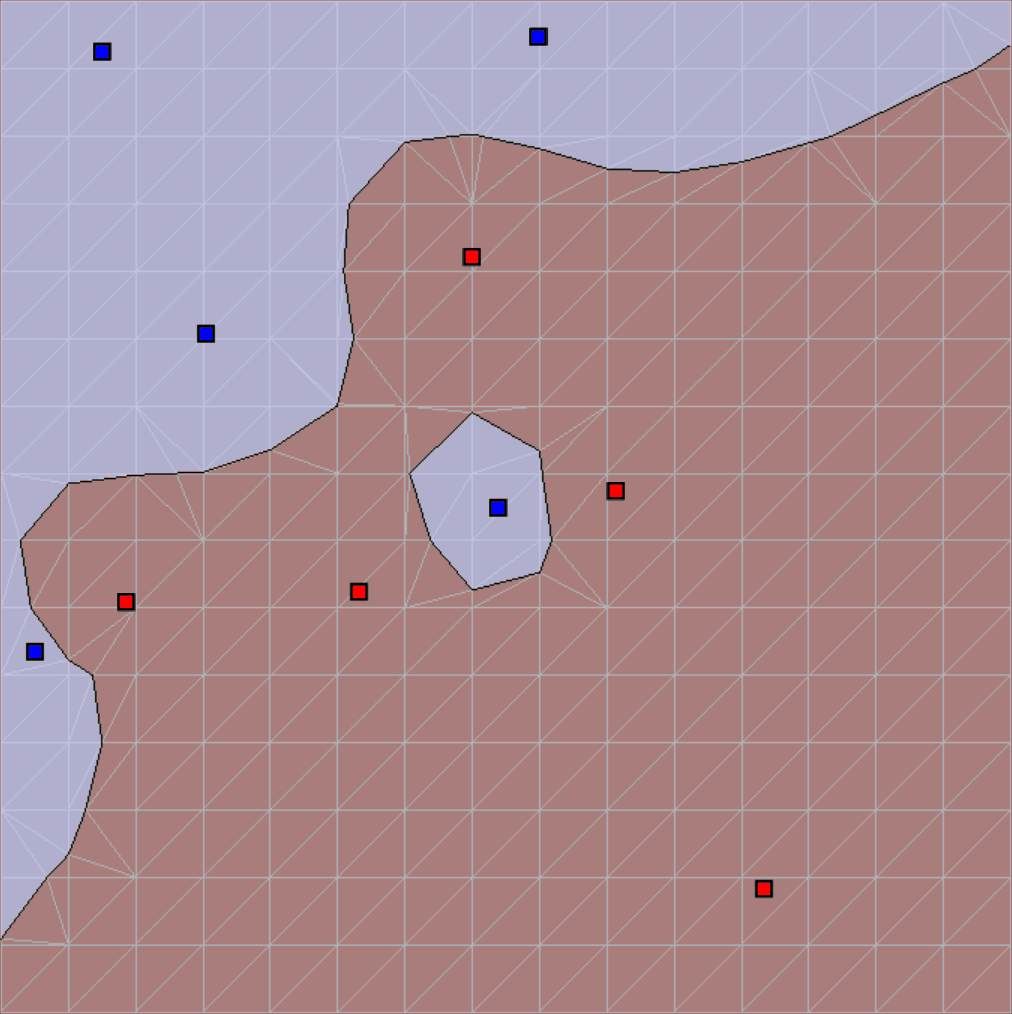
\includegraphics[width = 3 in]{16_res.png}
  \caption{The output of the Marching Squares algorithm: curvilinear, radial separation. Grid resolution is 16x16.
}
\end{figure}



\begin{figure} 
\centering
  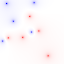
\includegraphics[width = 3 in]{64_res_image.png}
  \caption{Bitmap image used as input to the Marching Squares algorithm. 
Image size is 64x64.
}
\end{figure}

\begin{figure} 
\centering
  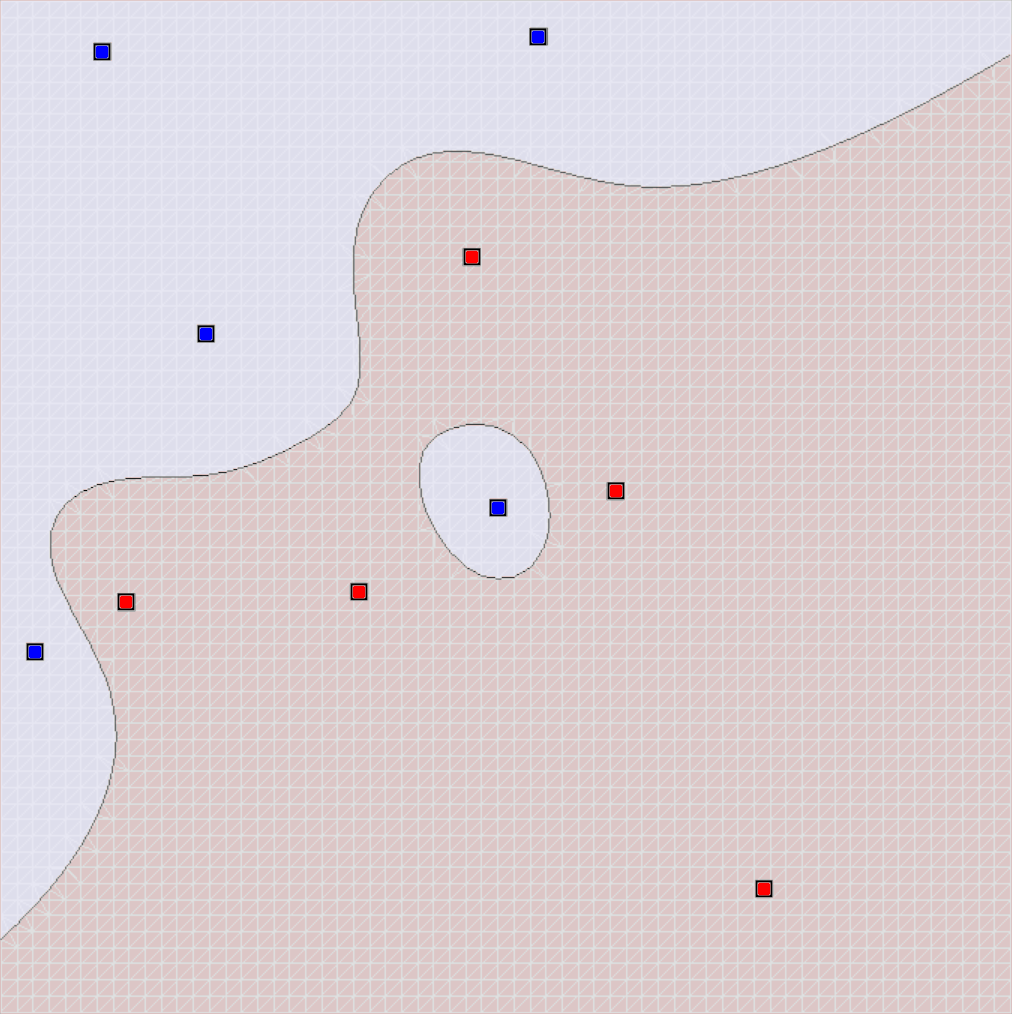
\includegraphics[width = 3 in]{64_res.png}
  \caption{The output of the Marching Squares algorithm: curvilinear, radial separation. Grid resolution is 64x64.
}
\end{figure}







\begin{figure} 
\centering
  
\includegraphics[width = 3 in]{image_avg_rectilinear.png}
  \caption{Bitmap image used as input to the Marching Squares algorithm.
Image size is 2x2.
}
\end{figure}

\begin{figure} 
\centering
  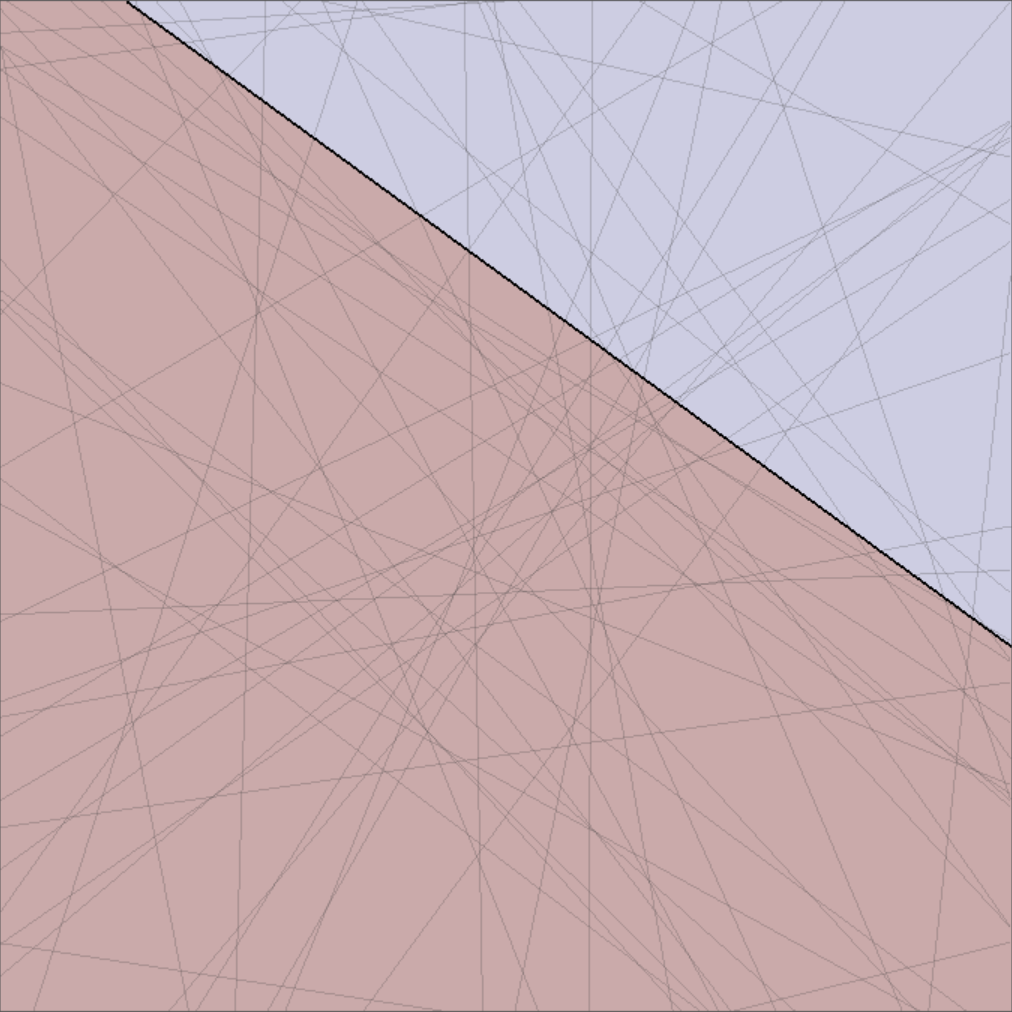
\includegraphics[width = 3 in]{rectilinear.png}
  \caption{The output of the Marching Squares algorithm: rectilinear separation. 
Grid resolution is 2x2.
All 50 contour sets have been drawn in transparent grey, with the exception of the average contour set, which is drawn in pure black.
}
\end{figure}



\begin{figure} 
\centering
  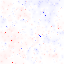
\includegraphics[width = 3 in]{image_avg_no_blur.png}
  \caption{Bitmap image used as input to the Marching Squares algorithm.
Image size is 64x64.
}
\end{figure}

\begin{figure} 
\centering
  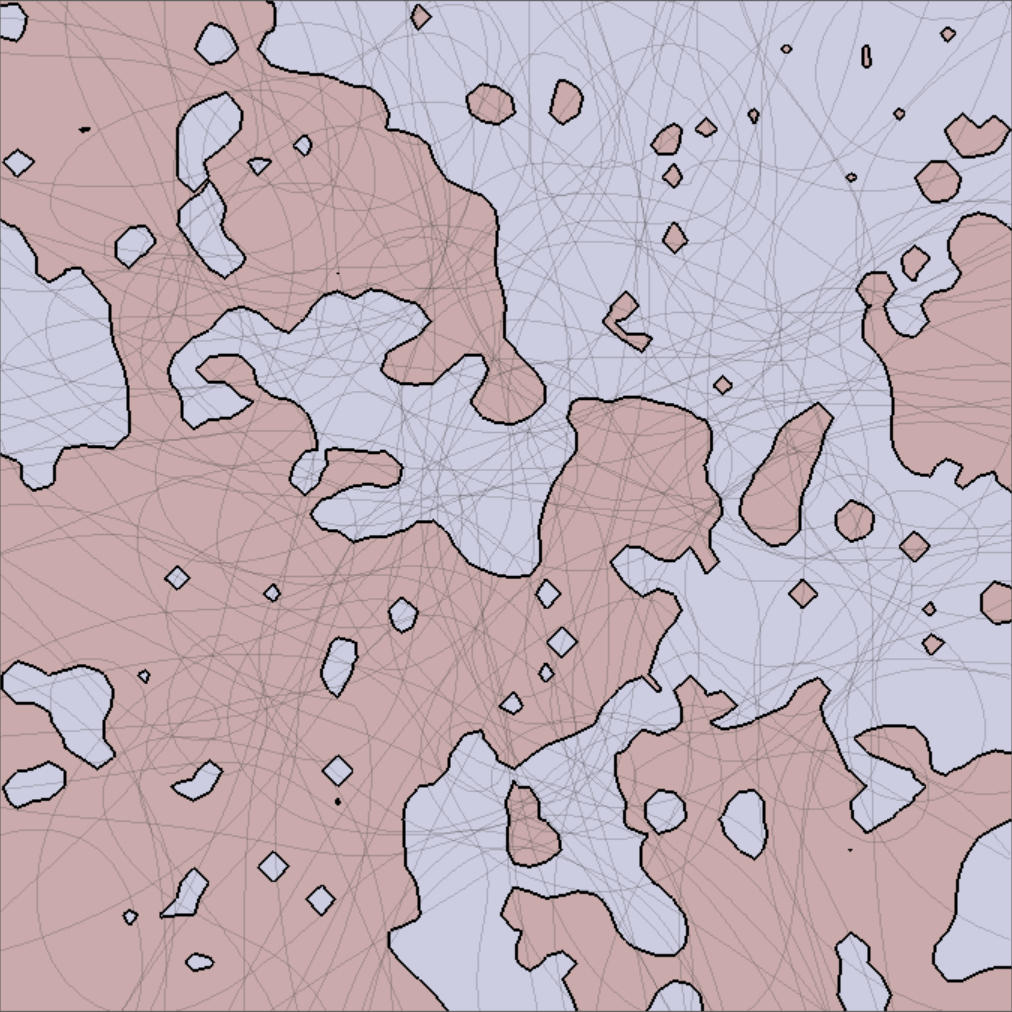
\includegraphics[width = 3 in]{no_blur.png}
  \caption{The output of the Marching Squares algorithm: curvilinear, radial separation. 
Grid resolution is 64x64.
All 50 contour sets have been drawn in transparent grey, with the exception of the average contour set, which is drawn in pure black.
}
\end{figure}





\begin{figure} 
\centering
  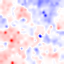
\includegraphics[width = 3 in]{image_avg_1blur.png}
  \caption{Bitmap image used as input to the Marching Squares algorithm.
Image size is 64x64.
One iteration of Gaussian blur has been used.
}
\end{figure}


\begin{figure} 
\centering
  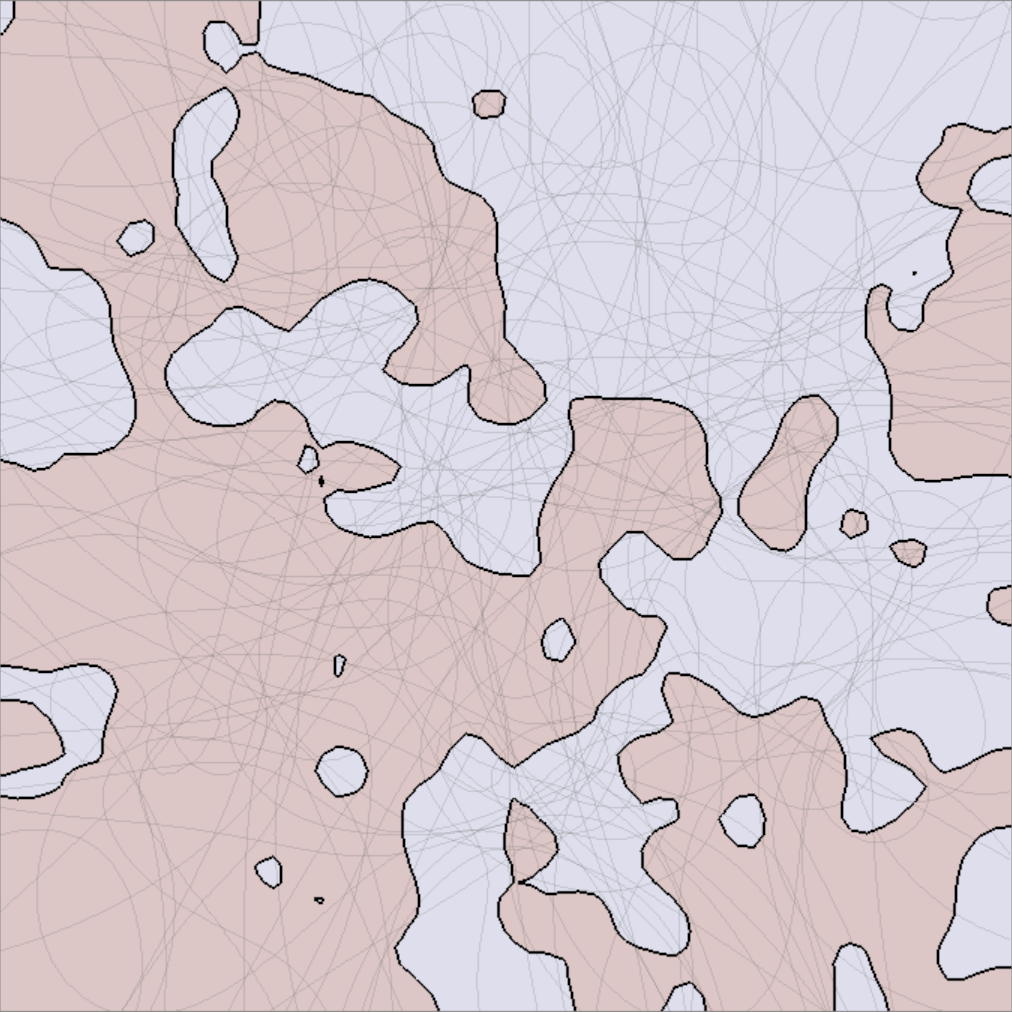
\includegraphics[width = 3 in]{1blur.png}
  \caption{The output of the Marching Squares algorithm: curvilinear, radial separation. 
Grid resolution is 64x64.
All 50 contour sets have been drawn in transparent grey, with the exception of the average contour set, which is drawn in pure black.
}
\end{figure}







\begin{figure} 
\centering
  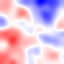
\includegraphics[width = 3 in]{image_avg_10blur.png}
  \caption{Bitmap image used as input to the Marching Squares algorithm.
Image size is 64x64.
Ten iterations of Gaussian blur have been used.
}
\end{figure}
	
\begin{figure} 
\centering
  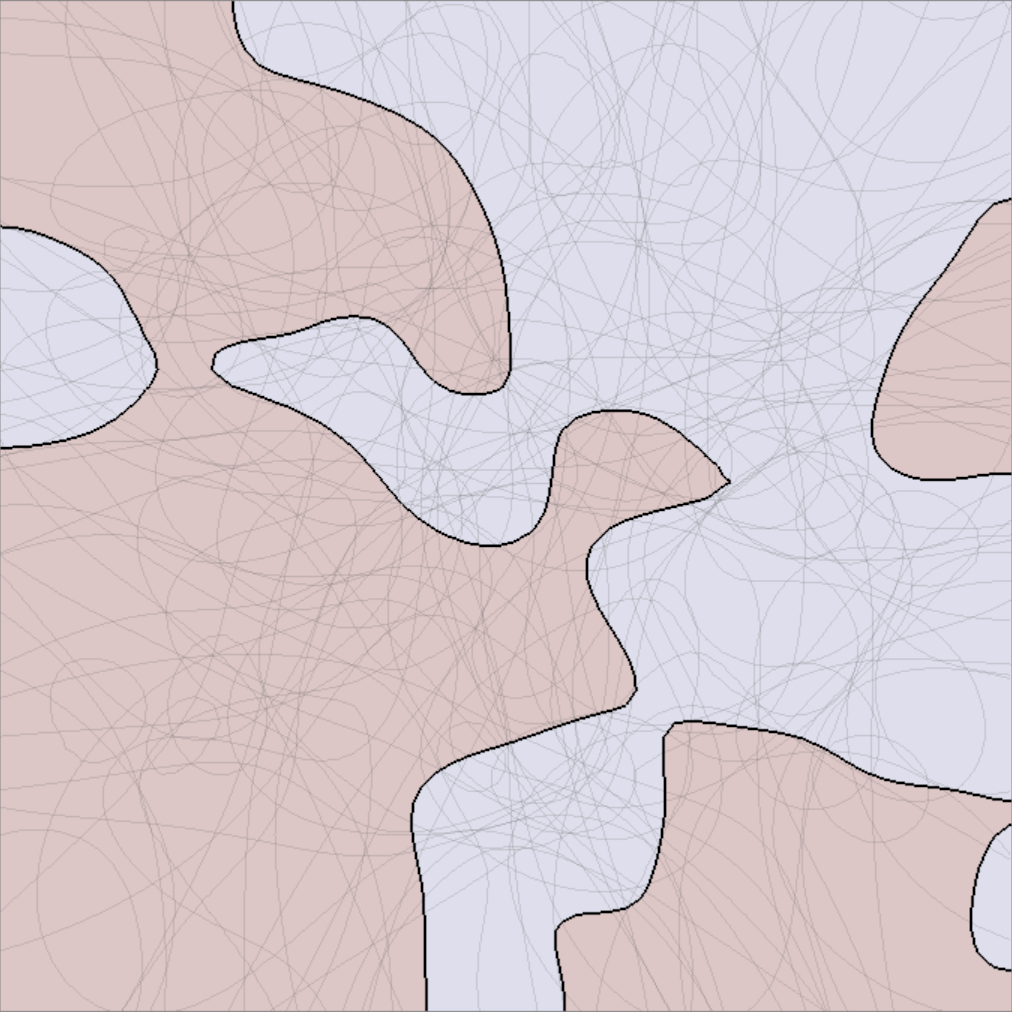
\includegraphics[width = 3 in]{10blur.png}
  \caption{The output of the Marching Squares algorithm: curvilinear, radial separation. 
Grid resolution is 64x64.
All 50 contour sets have been drawn in transparent grey, with the exception of the average contour set, which is drawn in pure black.
}
\end{figure}





\end{document}









